\documentclass[10pt]{article}
\usepackage[polish]{babel}
\usepackage[utf8]{inputenc}
\usepackage[T1]{fontenc}
\usepackage{amsmath}
\usepackage{amsfonts}
\usepackage{amssymb}
\usepackage[version=4]{mhchem}
\usepackage{stmaryrd}
\usepackage{graphicx}
\usepackage[export]{adjustbox}
\graphicspath{ {./images/} }

\title{GIMNAZJUM }

\author{}
\date{}


\begin{document}
\maketitle
\begin{enumerate}
  \item W trapezie równoramiennym \(A B C D\), w którym \(A B=C D\), opuszczono wysokość \(B H\) i poprowadzono przekątną \(B D\). Przekątna ta jest dwusieczną kąta \(C D A\). Udowodnij, że kąt \(H B D\) jest równy sumie kątów \(A B H\) i \(C B D\).\\
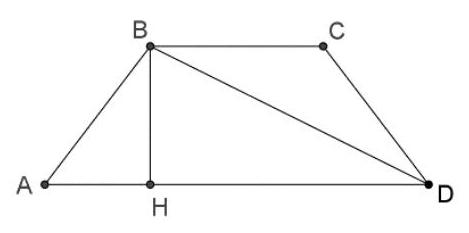
\includegraphics[max width=\textwidth, center]{2024_11_21_17a8ac2904543f8d31ceg-1(2)}
  \item Która liczba jest większa \(3^{100}-2^{150}\) czy \(3^{50}+2^{75}\) ?
  \item Znajdź takie dwie liczby \(a\) i \(b\), aby
\end{enumerate}

\[
a+b=a \cdot b=\frac{a}{b}
\]

\section*{LICEUM}
\begin{enumerate}
  \item Wewnątrz kwadratu \(A B C D\) obrano punkt \(M\) w równej odległości od boku \(C D\) i od wierzchołków \(A\) i \(B\). Jaką część pola kwadratu stanowi pole trójkąta \(A B M\) ?
  \item Oblicz \(\sqrt{\underbrace{11 \ldots 1}_{2 n}-\underbrace{22 \ldots 2}_{n}}\)\\
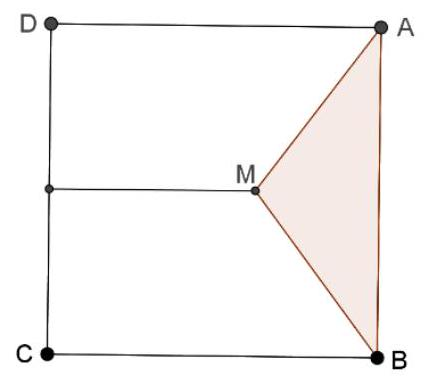
\includegraphics[max width=\textwidth, center]{2024_11_21_17a8ac2904543f8d31ceg-1(1)}
  \item Ile wynosi suma liczb n-tego wiersza trójkątnej tablicy:\\
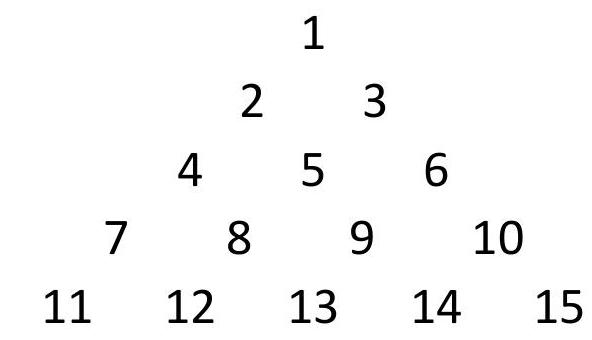
\includegraphics[max width=\textwidth, center]{2024_11_21_17a8ac2904543f8d31ceg-1}
\end{enumerate}

Odpowiedź uzasadnij.


\end{document}